
\section{{\prg mcdisp} - the Calculation Program for Magnetic Excitations}\label{mcdisp}

For a given field $\mbf H$ and temperature $T$ the dynamics of the magnetic system
can be calculated by the program {\prg mcdisp\index{mcdisp}}, for details
on the theory see appendix~\ref{formalism}. {\prg mcdisp\index{mcdisp}} requires as input files
the {\prg mcphas.j\index{mcphas.j}} and single ion input files. In addition, the input file
{\prg mcdisp.par\index{mcdisp.par}} and {\prg mcdisp.mf\index{mcdisp.mf}} are needed 
(see description below). 

\begin{description}
\item [\prg mcdisp [options]][file.mf]]  
      calculates the dispersion of magnetic excitations
	  needs as input file a {\prg file.mf} (default {\prg mcdisp.mf\index{mcdisp.mf}})
				and {\prg mcdisp.par\index{mcdisp.par}}.  Creates  
				files {\prg ./results/mcdisp.qom} and {\prg ./results/mcdisp.qei}
				containing the dispersion of the magnetic excitations and the neutron
				scattering intensity. 
				
				Options are:
				 \begin{itemize}
				\item Option {\prg -max} restricts the single ion susceptibility
				used to maximum of  the n lowest lying transitions, starting
				from the ground state (useful to save calculation time).
--
			        Note that by options {\prg -minE} and {\prg -maxE}
				also an energy interval may be given (minE,maxE):
				Single ion transitions with energies outside this
				energy interval are not considered.
                                               \item option {\prg -d} forces mcdisp to do calculation of intensities in dipole approximation only				
				\item Option {\prg -r} is used to calculate the energy dependence
				of the cross section via the direct evaluation of the
 dynamical susceptibility for a set of energy values (see appendix~\ref{formalism}). 
If option {\prg -r 0.032} is used, the energy dependence of 
the scattering cross section is calculated within limits [emin,emax] (given in file
{\prg mcdisp.par}).
The number, 0.032 in our case, indicates the imaginary part of $\omega$ 
in units of meV (see equations
in section~\ref{formalism}). Setting it zero would lead to numerical
divergencies, choosing it to large leads to large half widths of the calculated 
peaks. 
 Output
is stored in output file {\prg mcdisp.dsigma}.
{\em Note}: option {\prg -r} will only work correctly if all the single ion modules
which are used conform to the following convention: if $g_J\neq0$, then 
$\hat I_1=\hat J_x,\hat I_2=\hat J_y,\hat I_3=\hat J_z$, 
if $g_J=0$ then $\hat I_1=\hat S_x, \hat I_2=\hat L_x, \hat I_3=\hat S_y, \hat I_4=\hat L_y,
\hat I_5=\hat S_z,\hat  I_6=\hat L_z$ (here $\hat \mbf S, \hat \mbf L,\hat \mbf J$ refer to the
spin-, orbital- and total angular momentum, respectively in a coordinate system where
$y||b$,$z||(a \times b)$ and $x$ perpendicular to $y$ and $z$).
				\item To create an output
				of the Fourier transform ${\mathcal J}({\mbf Q})$ use option
				{\prg -jq} (outputs largest eigenvalue of ${\mathcal J}({\mbf Q})$ and 
corresponding eigenvector) or option {\prg -jqe} (outputs all eigenvalues). 
If energies are given for hkls in mcdisp.par, output file mcdisp\_scaled.jq contains scaled parameters
such that energy of first hkl set corresponds to highest eigenvalue of ${\mathcal J}({\mbf Q})$.
				\item {\prg -v} option is to display\index{display} more information.
                                
				\item Option {\prg -a} can be used to avoid overwriting output files in results, new results
				are appended.
								
				\item Option {\prg -c}  can be used to create  a single ion
				transition file {\prg ./results/mcdisp.trs}, which contains
				all single ion transitions used in the calculation. It also contains the 
                                    neutron intensities of the non interacting subsystems. This file can
				be edited (uncommenting single ion transitions which should not
				by used by a \# sign at the beginning of the line)
				and then the program can be restarted using the 
				\item  option {\prg -t} to
				read the single ion transition file {\prg ./results/mcdisp.trs} and
				calculate energies and neutron intensities of dispersive modes.
				\item Option {\prg -ninit n} to set the maximum number of low lying
                                 initial states, which will be considered in calculating a single ion susceptibility (not functional
                                 in all single ion modules).
 \item Option {\prg -pinit p} to set the minimum thermal population of a 
                                 initial state in order to be considered in the singleion ion susceptibility (not functional in
                                 all singleion ion modules).
 \item Option {\prg -prefix 001} to allow for easy parallel processing: all output files {\prg results/mcdisp.*}
                  will then be created with prefix {\prg 001}, i.e. {\prg results/001mcdisp.*}.
                  Moreover,  in {\prg mcdisp.par} it is then possible to enter
                  variables like {\prg hklline=}  with prefix, in our case {\prg 001}, i.e. {\prg 001hklline}: this will trigger
                  the program to read these variables only if started with the option {\prg -prefix 001}. Another process
                  maybe started with {\prg -prefix 002} and will read variables such as {\prg 002hklline} and ignore {\prg 001hklline}.
                  Variables without prefixes will always be read and used.
                  After finishing the different processes, the results of the calculations stored e.g. in {\prg 001mcdisp.qei} and
                  {\prg 002mcdisp.qei} may be merged by commands like {\prg appendfile mcdisp.qei 001mcdisp.qei 002mcdisp.qei}.
    \item Option {\prg -ignore\_not\_posdef\_matrix\_error} ignores error when energies get complex due to unphysical mf groundstate.
    \item Option {\prg -x} to calculate resonant inelastic x-ray intensities (maximized with respect to azimuth) instead of neutron intensities.
    \item Option {\prg -xa  azstp} to calculate resonant inelastic x-ray intensities with complete azimuth dependence for each reflection in steps azstep (deg).
    \item Option {\prg -xaf  azimuth} to calculate resonant inelastic x-ray intensities for the given azimuth (deg).
				\end{itemize}
\item [\prg mcdispit [options]][file.mf]]  same as {\prg mcdisp}, but no graphic window
\end{description} 

\subparagraph{example of input file {\prg  mcdisp.mf}}
this file contains temperature $T$, the external field $H$ and
the exchange fields on the different sites:

\begin{verbatim}
# Parameter file  mcdisp.mf - read by mcdisp version 3.0
#<!--mcdisp.mcdisp.mf>
#*********************************************************************
# mcdisp - program to calculate the dispersion of magnetic excitations
# reference: M. Rotter et al. J. Appl. Phys. A74 (2002) 5751
#*********************************************************************
#'T'             temperature T
#'Ha' 'Hb' 'Hc'  magnetic field
#'n'             number of atoms in magnetic unit cell
#'nofatoms'      number of atoms in primitive crystal unit cell
#'nofcomponents' dimension of moment vector of a magnetic atoms
T=2 Ha=0 Hb=0 Hc=0 n=10 nofatoms=2 nofcomponents=3
 0.0000 0.0000 0.0000 0.0000 0.0000 0.0000 0.0000 0.0000 0.0000 0.0000
 0.2708 0.3354 -0.3354 -0.2708 0.2947 -0.2708 -0.3354 0.3354 0.2708 -0.2947
 0.0000 0.0000 0.0000 0.0000 0.0000 0.0000 0.0000 0.0000 0.0000 0.0000
 0.0000 0.0000 0.0000 0.0000 0.0000 0.0000 0.0000 0.0000 0.0000 0.0000
 0.2708 0.3354 -0.3354 -0.2708 0.2947 -0.2708 -0.3354 0.3354 0.2708 -0.2947
 0.0000 0.0000 0.0000 0.0000 0.0000 0.0000 0.0000 0.0000 0.0000 0.0000
\end{verbatim}

The file {\prg mcdisp.mf\index{mcdisp.mf}} can be easily set up by using the program {\prg %%@
setup\_mcdisp\_mf\index{setup\_mcdisp\_mf}} or alternatively by the program {\prg spins\index{spins}} 
described in section~\ref{displaydensities}.
                            Note, in case of non-orthogonal axes the convention for applied field $Ha, Hb,Hc$                     
                            is $Hb||\vec b$, $Hc||(\vec a \times \vec b)$ and $Ha$ perpendicular to $Hb$ and $Hc$.

\subparagraph{example of input file {\prg mcdisp.par\index{mcdisp.par}}}

{\footnotesize
\begin{verbatim}
# Parameter file  mcdisp.par - read by mcdisp version 5.1
#<!--mcdisp.mcdisp.par>
#*********************************************************************
# mcdisp - program to calculate the dispersion of magnetic excitations
# reference: M. Rotter et al. J. Appl. Phys. A74 (2002) 5751
#*********************************************************************
#
# mcdisp calculates the neutron scattering cross section dsigma/dOmegadE' [barn/sr/meV/f.u.]
#           f.u.=crystallogrpaphic unit cell (r1xr2xr3) for inelastic and diffuse scattering
#
# depending on what is kept constant it follows either kf or ki (1/A)
#!kf=3.474
# 
# emin and emax define the energy range in which neutron intensities are calculated
# for full calculation of the dynamical susceptibility (option "-r", inversion of the MF-RPA equation 
# for each point in Q-omega space) the minimum and maximum energy has to be given (energy stepwidth is 
# equal to the parameter epsilon given in the command line after "-r")
#
#!emin=0.1
#!emax=80
#
# optional switches which can be 0 or 1 are
#!calculate_magmoment_oscillation=1  creates mcdisp.qem
#!calculate_spinmoment_oscillation=0  creates mcdisp.qes
#!calculate_orbmoment_oscillation=0  creates mcdisp.qeo
#!calculate_chargedensity_oscillation=1  creates mcdisp.qee
#!calculate_spindensity_oscillation=0  creates mcdisp.qsd
#!calculate_orbmomdensity_oscillation=0  creates mcdisp.qod
#!calculate_phonon_oscillation=0  creates mcdisp.qep
#
# (optional) number of parallel threads on your machine
#  (if not set program will attempt to determine this automatically)
# nofthreads=2
#
#     out* controls the type of output in user defined columns in files mcdisp.qei,qex,qom,dsigma,dsigma.tot
#!out1=1 
#!out2=6 
#!out3=7 
#!out4=4 
#     ... in out*=n the numbers n have the following meaning:
#            0....Qinc[1/A] 
#            1....Qx[1/A]   
#            2....Qy[1/A]   
#            3....Qz[1/A]   
#            4....T[K]      
#            5....Ha[T]     
#            6....Hb[T]     
#            7....Hc[T]     
#            8....|Q|[1/A]  
#
# optional switch outS for control of the output of the magnetic scattering function in results/mcdisp.qei
#! outS=3
# .. valid values are
# 0: not output of Salphabeta
# 1: output Sperpalphabeta(Q,omega) in dipole approximation, with alpha,beta=x,y,z
# 2: output Sperpalphabeta(Q,omega) going beyond dipole approximation (if possible), with alpha,beta=x,y,z
# 3: output Sperpalphabeta(Q,omega) in dipole approximation, with alpha,beta=u,v,w
# 4: output Sperpalphabeta(Q,omega) going beyond dipole approximation (if possible), with alpha,beta=u,v,w
# 5: output Salphabeta(Q,omega) in dipole approximation, with alpha,beta=x,y,z (no output of dip intensity)
# 6: output Salphabeta(Q,omega) in dipole approximation, with alpha,beta=u,v,w (no output of dip intensity)
#
# xyz coordinate refer to y||b, z||(a x b) and x normal to y and z
# uvw coordinates refer to u||Q=k-k', w perpendicular to the scattering plane
#     (as determined by the cross product of subsequent vectors in the input
#     q-vector list) and v perpendicular to u and w, such that uvw form a righthanded system
#
#
# Commands such as the following are used to generate a hkl list (to activate put #! instead of # at beginning of line):
#
# - a Q vector mesh to be mapped in the calculation it can be in Miller indices
#hmin=0 hmax=1 deltah=0.1
#kmin=0 kmax=1 deltak=0.1
#lmin=0 lmax=1 deltal=0.1
#
# or in Qx Qy Qz (1/A) where y||b z||axb and x perpendicular to y and z
#Qxmin=0 Qxmax=1 deltaQx=0.1
#Qymin=0 Qymax=1 deltaQy=0.1
#Qzmin=0 Qzmax=1 deltaQz=0.1
#
# - file(s) containing list of Q vectors with (optional) energies of observed excitations to be fitted
# h k l [E(meV) [statistical_weight  [intensity [fwhm ]]]]
#
# hklfile=file1
# hklfile=file2
# ...
#
# or
# Qx Qy Qz(1/A) [E(meV) [statistical_weight  [intensity [fwhm ]]]]
#
# QxQyQzfile=file1
# QxQyQzfile=file2
# ...
#
#
# - some lines in reciprocal space 
#
#hklline=h1=0 k1=1 l1=0 to hN=1 kN=1 lN=0 Nstp=21
#hklline=h1=0 k1=2 l1=0 to hN=1 kN=1 lN=0 Nstp=21
#
#QxQyQzline=Qx1=0 Qy1=1 Qz1=0 to QxN=1 QyN=1 QzN=0 Nstp=21
#QxQyQzline=Qx1=0 Qy1=2 Qz1=0 to QxN=1 QyN=1 QzN=0 Nstp=21
#
# - some planes in reciprocal space 
#
#hklplane=h0=0 k0=1 l0=0 to hN=1 kN=1 lN=0 Nstp=21 to hM=1 kM=0 lM=3 Mstp=21  
# or
#QxyQzplane=Qx0=0 Qy0=1 Qz0=0 to QxN=1 QyN=1 QzN=0 Nstp=21 to QxM=1 QyM=0 QzM=3 Mstp=21  
# 
#
# - a list of Q vectors with (optional) energies of observed excitations to be fitted
# h k l [E(meV) [statistical_weight  [intensity [fwhm ]]]]
1 0 0 
2 0 0 
3 0 0 
0.1 0 0 
0 0.1 0 
0 0 0.1 

\end{verbatim}
}

this file describes, which $q$ vectors will be calculated.
Miller indices always refer to the lattice $\vec a^*, \vec b^*, \vec c^*$, which
is the reciprocal lattice of $\vec a, \vec b, \vec c$ as defined by lattice
parameters $a,b,c$ and angles $\alpha,\beta,\gamma$ as given in
input file {\prg mcphas.j}.


The
program {\prg mcdisp\index{mcdisp}} then calculates only 
the excitation energies at these reflections and (if measured
energies are given) computes a standard deviation
and prints
this deviation to stdout as ''sta=3120.31'' [this can directly
be used by fitting program such as {\prg simannfit\index{simannfit}}].

The standard deviation is calculated by taking for a set of measured energies (at a 
given q-vector) the squared sum of differences to the nearest
calculated energy. Statistical weighting as given by the user in {\prg mcdisp.par}
for each q-vector is applied. If the weighting is less than zero, the 
inverse squared sum of differences to the nearest
calculated energy is taken (''antipeak'', this is useful in order to 
tell the program, that there is no peak at this energy).
In addition to the standard deviation ''sta'' some other quantitites are calculated and 
may be used in fitting experimental data:

\begin{eqnarray}
{\rm sta}                              & =& \sum_i |weight(i)|*[Eexp(i) - nearestEcalc(i)]^{[2*sign(weight(i))]}\\
{\rm sta\_int   }                       & = &\sum_i |weight(i)|*[Eexp(i) - nearestEcalc_{\rm with %%@
Int>0.1mb/srf.u.}]^{[2*sign(weight(i))]}\\
{\rm sta\_without\_antipeaks }           & =& \sum_{i, weight(i)>0}  weight(i)*[Eexp(i) - nearestEcalc(i)]^2\\
{\rm sta\_int\_without\_antipeaks }       & =&\sum_{i,weight(i)>0}  weight(i)*[Eexp(i) - nearestEcalc_{\rm with %%@
Int>0.1mb/srf.u.}]^2\\
{\rm sta\_without\_weights }              &=& \sum_i [Eexp(i) - nearestEcalc(i)]^{[2*sign(weight(i))]}\\
{\rm sta\_int\_without\_weights}          & =&\sum_i [Eexp(i) - nearestEcalc_{\rm with %%@
Int>0.1mb/srf.u.}]^{[2*sign(weight(i))]}\\
{\rm sta\_without\_antipeaks\_weights}    & = &\sum_{i, weight(i)>0}[Eexp(i) - nearestEcalc(i)]^2\\
{\rm sta\_int\_without\_antipeaks\_weights}& =& \sum_{i, weight(i)>0} [Eexp(i) - nearestEcalc_{\rm with %%@
Int>0.1mb/srf.u.}]^2\\
\end{eqnarray}




The output files of program {\prg McDisp} are 

\begin{quote}
\item[{\prg mcdisp.trs}:] contains all single ion transitions with strengths $\gamma$ 
and neutron intensities.
\item [{\prg mcdisp.qom}:] Contains the energies of the modes and scattering cross sections  for each mode 
calculated using the DMD algorithm described in section~\ref{DMDform}
\item[{\prg mcdisp.qei}] energies and neutron scattering intensities calculated by the DMD algorithm, if 
        the energy of a mode is outside interval  [emin,emax] the value -1 is output for the intensity.
\item[{\prg mcdisp.qem .qes .qel .qsd .qod .qee}] eigenvectors for different observables (relative phase and amplitudes)
\item [{\prg mcdisp.dsigma}(only created with option {\prg -r}):] Contains the energy dependence of the scattering cross %%@
section
calculated according to section~\ref{formalism} within the energy range specified by [emin,emax] given in {\prg %%@
mcdisp.par}. 
\item [{\prg mcdisp.dsigma.tot}:] sum of intensities in interval  [emin,emax].  For option {\prg -r} : Sum of intensities calculated in {\prg %%@
mcdisp.dsigma}.
\end{quote}

\vspace{1cm}
{\em Exercises:}
\begin{itemize}
\item Type {\prg mcdisp -max 3} to
calculate the dispersion of magnetic excitations for NdCu$_2$.
and inspect the results
{\prg examples/ndcu2b\_new/results/mcdisp.qei}.
Which  transition has the largest intensity ?
\end{itemize}

\subsection{Viewing the results of McDisp}

\begin{quote}
\item [\prg displaybubbles\index{displaybubbles} ] produces a plot of the calculated dispersion on screen, which is 
                       automatically updated when the file changes. In contrast to the normal
		       display\index{display} program the radius of the symbols is increased according to
		       the values of a radius column (in our case intensity column in file
		       mcdisp.qui). Use as {\prg displaybubbles\index{displaybubbles} 
		       xcol ycol rcol filename} - i.e. for displaying the dispersion along
		       {\em h} type {\prg displaybubbles\index{displaybubbles}  5 8 9 mcdisp.qei}. 
\item [\prg displaycontour\index{displaycontour}] displays contour plot of scattering intensity - use as
                       {\prg displaycontour\index{displaycontour} xcol ycol zcol filename} - i.e. for displaying
		       the intensity versus {\em hk} type {\prg displaycontour\index{displaycontour} 5 6 8 mcdisp.dsigma.tot}
		       (see fig.~\ref{ho2ti2o7diffuse})
\item [\prg spectrum]  reads mcdisp.qom or mcdisp.dsigma and produces spectrum
                       as an xy file, use as {\prg spectrum h k l filename}
\item [\prg display\_densities\index{display\_densities}] produces an animation of the 
                       oscillation of spin, magmoments, chargedensity,... see also
                       section~\ref{displaydensities} and appendix~\ref{visualization}.
\end{quote}






\begin{figure}[t]%h=here, t=top, b=bottom, p=separate figure page
\begin{center}\leavevmode
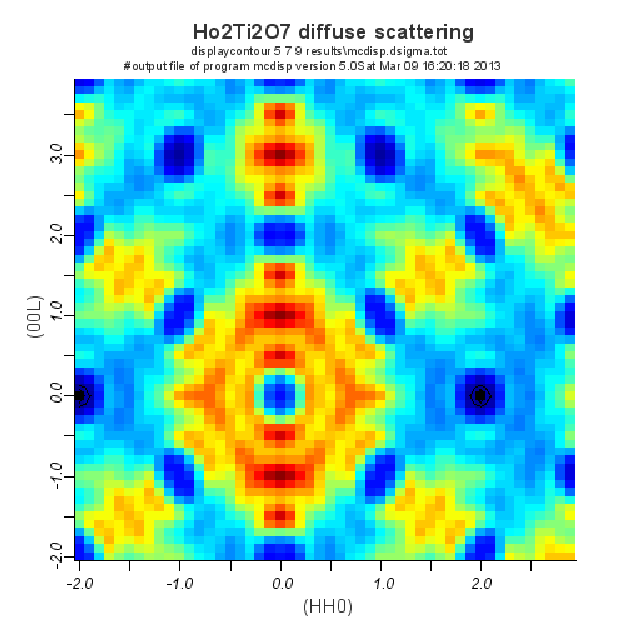
\includegraphics[angle=-0, width=0.6\textwidth]{figsrc/ho2ti2o7diffuse.eps}
\end{center}
\caption{\label{ho2ti2o7diffuse}
Ho$_2$Ti$_2$O$_7$ - calculated diffuse magnetic scattering intensity in the (110)-(001)
 plane at $T=10$~K.
[plot created by program {\prg displaycontour\index{displaycontour}}]
}
\end{figure}

\subsection{Diffuse Scattering}

The program {\prg McDisp} may be used straightforward to calculate quasi elastic intensity
 by

\begin{itemize}
\item
 specification of an energy
range [emin,emax] in file {\prg mcdisp.par\index{mcdisp.par}} which corresponds to the interval of energies (around zero
energy transfer) sensed by the detector of the diffuse scattering experiment. 
\item
 quasi elastic intensity is expected only in the paramagnetic state - thus in {\prg mcdisp.mf\index{mcdisp.mf}} a
 a temperature above the magnetic ordering temperature should be selected.
\item start {\prg mcdisp} in the usual way, using the DMD method.
\end{itemize} 
 
The file {\prg mcdisp.dsigma.tot} produced by the calculation contains the calculated diffuse scattering cross section.
Figure~\ref{ho2ti2o7diffuse} shows an output of such a calculation for the diffuse scattering
on Ho$_2$Ti$_2$O$_7$.

For comparison it is also possible to do a calculation using the option {\prg -r} forcing
 the program {\prg mcdisp\index{mcdisp}} to calculate the cross section
 using the full MF-RPA algorithm (output stored in {\prg mcdisp.dsigma})

\subsection{Powder Neutron Cross Section}


\begin{figure}[tb]%h=here, t=top, b=bottom, p=separate figure page
\begin{center}\leavevmode
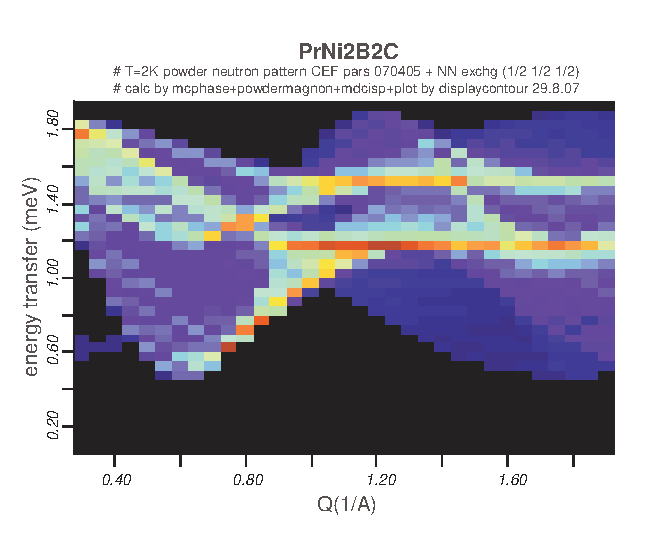
\includegraphics[angle=0, width=0.5\textwidth]{figsrc/contour2K_070504.eps}
\end{center}
\caption{Magnetic Neutron powder spectrum of PrNi$_2$B$_2$C for $T=2$~K as calculated using module {\prg powdermagnons} %%@
in combination with {\prg 
mcdisp}.}\label{prni2b2c_2K}
\end{figure}

\begin{figure}[tb]%h=here, t=top, b=bottom, p=separate figure page
\begin{center}\leavevmode
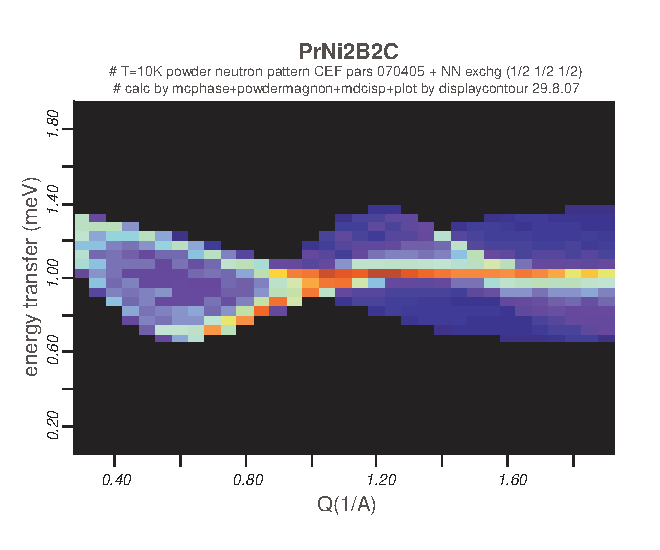
\includegraphics[angle=0, width=0.5\textwidth]{figsrc/contour10K_070504.eps}
\end{center}
\caption{Magnetic Neutron powder spectrum of PrNi$_2$B$_2$C for $T=10$~K  as calculated using module {\prg %%@
powdermagnons} in combination with {\prg 
mcdisp}.}\label{prni2b2c_10K}
\end{figure}

{\prg Mcdisp} in combination with module {\prg powdermagnon} can be used to calculate
powder neutron pattern. In order to do this, a 3-step procedure is required:

\subsubsection{Creation of the q-vector list}
The first step is to create a list of reflections to be used for 
the averaging of the powder neutron cross section. 

just type: powdermagnon 0.3 2 0.1 80

meaning take file {\prg mcphas.j\index{mcphas.j}}, generate a reflection list and put it to 
file {\prg mcdisp.par\index{mcdisp.par}}. Parameters in the above command are 
\begin{itemize}
\item
 0.3 ....qmin   [1/A] minimal q vector
\item
 2   ....qmax   [1/A] maximal q vector
\item
 0.1 ....deltaq [1/A] step width in q
\item
 80  ....number of steps in polar coordinate $\Theta$
        (steps in polar angle $\phi$ are  then calculated in module
        {\prg powdermagnon} by $\delta \phi= \delta \Theta*\pi/(4*sin(\Theta))$
\end{itemize}

\subsubsection{Calculation of the Dispersion using {\prg mcdisp\index{mcdisp}}}

In order to set the correct temperature and $k_f$ (or $k_i$) etc. edit
the input files for module {\prg mcdisp\index{mcdisp}} and start {\prg mcdisp\index{mcdisp}}. Mind 
to select the fast algorithm so that a file {\prg mcdisp.qei} is created.

\subsubsection{Powder-averaging the spectra}
The third and last step in the calculation of the powder pattern is the averaging
of the spectra with the same value of $Q$. This is done by restarting module
{\prg powdermagnon} by: 

powdermagnon -r results\\mcdisp.qei 0.5 30 0.2 

meaning take  results from file {\prg results\\mcdisp.qei} and average the
spectra. Output is printed to the console (STDOUT) and can be piped to a file in
order to print it with {\prg displaycontour\index{displaycontour}}. An example is given in fig.~
\ref{prni2b2c_2K} and \ref{prni2b2c_10K}.
Parameters in the above command  are:
\begin{itemize}
\item 0.5 ....Emin   [meV] minimal energy
\item 30 ....Emax   [meV] maximal energy
\item 0.2....deltaE [meV] energy step width
\end{itemize}


\subsection{Resonant Inelastic X-ray Scattering(RIXS)\index{RIXS}}

Using the option {\prg -x} and {\prg -xa}  the RIXS cross section can be calculated
by {\prg mcdisp}\index{mcdisp}. 
Option {\prg -x} calculates resonant inelastic x-ray intensities 
maximized with respect to azimuth.
 Option {\prg-xa}  calculates resonant inelastic x-ray 
intensities with complete azimuth dependence for each reflection.
		
The formalism is based on \cite[equ.8 ff]{haverkort10-167404},
e.g. the observables $\hat \mathcal O_{\alpha}$ are the 9 components ($\alpha$
=xx xy xz yx yy yz zx zy zz)
of the tensor $\mbf R$, which is related to the operator
$R_{\omega,j}^{\epsilon_i\epsilon_o}$ in \cite{haverkort10-167404} by

\begin{equation}
R_{\omega,j}^{\epsilon_i\epsilon_o}=\mbf \epsilon_o^{\star} \cdot \mbf R \cdot \mbf \epsilon_i
\end{equation}

Here the vector $\mbf \epsilon$ describes the polarisation of the incoming / outgoing
photon beam (linear (real) or circular polarized (complex) light).
Vector components (e.g. $\hat \mbf S$ to the xyz coordinate system, where
$y||b$,$z||(a \times b)$ and $x$ perpendicular to $y$ and $z$.

For the isotropic ion the scattering operator $R_{\omega,j}^{\epsilon_i\epsilon_o}$
is given by

\begin{eqnarray}\label{rixsop}
R_{\omega,j}^{\epsilon_i\epsilon_o}&=&\mbf \epsilon_o^{\star} \cdot \mbf R \cdot \mbf \epsilon_i \\
&=& \sigma^{(0)} \mbf \epsilon_i \cdot \mbf \epsilon_o^{\star} + \frac{\sigma^{(1)}}{s}
\mbf \epsilon_o^{\star} \times \mbf \epsilon_i \hat \mbf S_j \nonumber \\
&& \frac{\sigma^{(2)}}{s(2s-1)} \left ( 
\mbf \epsilon_i \cdot \hat \mbf S_j \mbf \epsilon_o^{\star} \cdot \hat \mbf S_j 
+ \mbf \epsilon_o^{\star} \cdot \hat \mbf S_j \mbf \epsilon_i \cdot \hat \mbf S_j  
- \frac{2}{3} \mbf \epsilon_i \cdot \mbf \epsilon_o^{\star} \hat \mbf S_j^2
\right )
\end{eqnarray}


In order to use this expression,  the conductivities $\sigma$ have
to be entered in the {\prg sipf} file, e.g.

\begin{verbatim}
SIGMA0r=1.32
SIGMA1r=1.32
SIGMA2r=1.32
SIGMA0i=1.32
SIGMA1i=1.32
SIGMA2i=1.32
\end{verbatim}
('r' and 'i' stand for real and imaginary part, respectively).

Note: in module {\prg so1ion}\index{so1ion} the scattering operator
is given in terms of the total angular momentum $\hat \mbf J$ instead
of $\hat \mbf S$.

If a more complex tensor $\mbf R$ is required, it's components
can be defined in the sipf file using the perlparse option.


\subsubsection*{Scattering geometry}

\begin{quote}
\item[Coordinate system, see\cite{longfield02-054417}:] Euclidean (orthonormal) system 
$[\mbf u_1,\mbf u_2,\mbf u_3]$. The scattering plane, defined by the
direction of the incident and final wave vectors  
$\mbf k$ and $\mbf k'$, contains $\mbf u_1$ lying
perpendicular and in the sense of $\mbf k$ and $\mbf u_3$ parallel to the scattering
vector $\mbf Q=\mbf k-\mbf k'$. 
\item[Polarisation of the Photon beam:] $\sigma$ and $\pi$ refer to the polarisation
of the beam parallel and perpendicular to $\mbf u2$, respectively.
\item[Angles for azimuth $\Psi=0$:] $\alpha_i=\angle(\mbf a_i \cdot \mbf u_3)_{\Psi=0}$,
$\delta_i=\angle(\mbf a_i^{\perp}\cdot \mbf u_1)_{\Psi=0}$,
where $\mbf a_{1,2,3}=\mbf a,\mbf b,\mbf c$ and $\mbf a_i^{\perp}$ is the projection of
$\mbf a_i$ onto the plane perpendicular to $\mbf Q$.
 In the chosen experimental geometry
azimuth $\Psi=0$, when $\mbf a_1 = \mbf a$ points to the x-ray source.
\end{quote}

